%-------------------------------------------------------------------------------------------
\documentclass[aspectratio=43,UTF8,10pt]{ctexbeamer}

%%%%%%%%%%%%%%%%%%%%%%%%%%%%%
\usepackage{colortbl}
\usepackage{color}
\usepackage{booktabs}
\usepackage{threeparttable}
\usepackage{hyperref}
%\usepackage{babel}
%%%%%%%%%%%%%%%%%%%%%%%%%%%%%

\mode<presentation> {
\usetheme{Madrid}
%\setbeamertemplate{footline} % To remove the footer line in all slides uncomment this line
\setbeamertemplate{footline}[frame number] % To replace the footer line in all slides with a simple slide count uncomment this line
\setbeamercolor{page number in head/foot}{fg=blue}
\setbeamertemplate{navigation symbols}{} % To remove the navigation symbols from the bottom of all slides uncomment this line
}

% User Defined Block %%%%%%%%%%%%%%%%%%%%%%%%%%%%%%%%%%%%%%%%%%%%%%%%%%%%%%%%
\usepackage{setspace}
\definecolor{orange}{rgb}{1,0.5,0}
\definecolor{aa}{RGB}{34,139,34}
\definecolor{lightblue}{rgb}{0,0.85,0.9}
\definecolor{darkblue}{rgb}{0,0.7,1}
\definecolor{hanblue}{rgb}{0.27, 0.42, 0.81}
\definecolor{indiagreen}{rgb}{0.07, 0.53, 0.03}
\definecolor{indianred}{rgb}{0.8, 0.36, 0.36}
\definecolor{indianyellow}{rgb}{0.89, 0.66, 0.34}
\definecolor{babypink}{rgb}{0.96, 0.76, 0.76}
\definecolor{ao(english)}{rgb}{0.0, 0.5, 0.0}
\definecolor{bondiblue}{rgb}{0.0, 0.58, 0.71}
\definecolor{ao(english)}{rgb}{0.0, 0.5, 0.0}
\definecolor{azure(colorwheel)}{rgb}{0.0, 0.5, 1.0}
\setbeamerfont{block title}{size=\normalsize}
\setbeamerfont{block body}{size=\small}

% User Defined Block %%%%%%%%%%%%%%%%%%%%%%%%%%%%%%%%%%%%%%%%%%%%%%%%%%%%%%%%
\newenvironment<>{abstractblock}[1]{%
  \setbeamercolor{block title}{fg=white,bg=bondiblue}%
%   \setbeamercolor{block body}{fg=white,bg=bondiblue}%
  \begin{block}#2{#1}}{\end{block}}
\newenvironment<>{blueblock}[1]{%
  \setbeamercolor{block title}{fg=white,bg=hanblue}%
  \begin{block}#2{#1}}{\end{block}}

\newenvironment<>{greenblock}[1]{%
  \setstretch{1.3}\setbeamercolor{block title}{fg=white,bg=indiagreen}%
  \begin{block}#2{#1}}{\end{block}}

\newenvironment<>{redblock}[1]{%
  \setstretch{1.3}\setbeamercolor{block title}{fg=white,bg=indianred}%
  \begin{block}#2{#1}}{\end{block}}

\newenvironment<>{yellowblock}[1]{%
  \setstretch{1.3}\setbeamercolor{block title}{fg=white,bg=indianyellow}%
  \begin{block}#2{#1}}{\end{block}}

%----------------------------------------------------------------------------------------
%	PACKAGES
%----------------------------------------------------------------------------------------
\usepackage{graphicx} % Allows including images
%\usepackage{tikz}
%\usetikzlibrary{shapes.geometric, arrows}
\usepackage{listings}
\lstset{language=C++,
    columns=flexible,
   % basicstyle=\scriptsize\ttfamily,                                      % 设定代码字体、大小4
    basicstyle=\footnotesize\ttfamily,
    %numbers=left,xleftmargin=2em,framexleftmargin=2em,                   % 在左侧显示行号
    %numberstyle=\color{darkgray},                                        % 设定行号格式
    keywordstyle=\color{blue},                                            % 设定关键字格式
    commentstyle=\color{ao(english)},                                     % 设置代码注释的格式
    stringstyle=\color{brown},                                            % 设置字符串格式
    %showstringspaces=false,                                              % 控制是否显示空格
	%frame=lines,                                                         % 控制外框
    breaklines,                                                           % 控制是否折行
    postbreak=\space,                                                     % 控制折行后显示的标识字符
    breakindent=5pt,                                                      % 控制折行后缩进数量
    emph={size\_t,array,deque,list,map,queue,set,stack,vector,string,pair,tuple}, % 非内置类型
    emphstyle={\color{teal}},
    escapeinside={(*@}{@*)},
    literate={&}{{\color{red}\&}}{1}                                      %{<replace>}{<replacement text>}{<length>} no comma between items
}
%---------------------------------------------------------------------------------------------------

%%%%%%%%%%%%%%%%%%%%%%%%%%%%%%%%%%%%%%%%%%%%%%%%%%%%%%%%%%%%%%%%%%%%%%%%%%%%%%%%%%%%%%%%%%%%%%
\title[\textit{C++程序设计}]{C++基础回顾}
%\author[李长河]{李长河} % Your name
%\institute[CUG] % Your institution as it will appear on the bottom of every slide, may be shorthand to save space
%{
%中国地质大学(武汉)自动化学院\\ % Your institution for the title page
%\medskip
%\textit{lichanghe@cug.edu.cn} % Your email address
%}
\date{} % Date, can be changed to a custom date
%%%%%%%%%%%%%%%%%%%%%%%%%%%%%%%%%%%%%%%%%%%%%%%%%%%%%%%%%%%%%%%%%%%%%%%%%%%%%%%%%%%%%%%%%%%%%%


\begin{document}

\begin{frame}[noframenumbering]           %beamer里重要的概念,每个frame定义一张page
\centering
{\large 面向对象软件开发技术 --人工智能 方向基础核心课程 \vspace{0.7cm} \\ 李长河 \vspace{0.5cm} \\自动化学院,信息楼710 \vspace{0.5cm}\\ lichanghe@cug.edu.cn}
\end{frame}

%-----------------------------------------------------------

\begin{frame}
\begin{columns}
	\begin{column}{0.6\textwidth}
	\begin{block}{教材}
	李长河, 童恒建, 叶亚琴等, C++程序设计(基于C++11标准). 电子工业出版社, \alert{2019年1月第2次印刷}
	\end{block}
\begin{block}{讲义和代码}
{\footnotesize \url{https://github.com/Changhe160/book-cplusplus}} \\
	\end{block}
\begin{block}{参考书}
	Stanley B. Lippman,Jos\'{e}e Lajoie,Barbara E. Moo.C++ Primer(第五版).王刚等译.北京:电子工业出版社,2013.	
	\end{block}
	\end{column}
	\hfill
	\begin{column}{0.35\textwidth}
		\begin{figure}[ht]
			\centering
			
\includegraphics[scale=0.8]{book.jpg}
		\end{figure}
	\end{column}
\end{columns}
\end{frame}


%-----------------------------------------------------------
\begin{frame}

\begin{block}{学习目标}
\begin{enumerate}
\item 掌握 {\color{red}面向对象}程序设计方法;
\item 运用常见 {\color{red}数据结构和算法}解决实际问题;
\item {\color{blue}熟悉可视化程序设计开发工具(Qt)。}
\end{enumerate}
\end{block}

\begin{block}<2->{课时安排}
讲课学时:28,实验学时:4(上机考试)
\end{block}

\begin{block}<3->{课程纪律}
\begin{enumerate}
\item 课上严禁看手机;
\item 课下作业和上机考试严禁抄袭,一经发现,均记0分处理。
\end{enumerate}
\end{block}

\begin{block}<4->{课程考核}
课程总成绩 = 考勤*5\%+四次作业*40\%+上机考试*40\%+ 课程报告*15\%
\end{block}
\end{frame}


%-----------------------------------------------------------
\begin{frame}

\begin{columns}
\begin{column}{0.8\textwidth}
    \begin{block}{统计联系方式}
    利用\alert{Excel}按照以下格式统计所有学生信息,\alert{班长}负责在\alert{下次上课前}发给我\\
       \vspace{0.2cm}
    姓名~~~~~~~~电子邮件\\
    李长河~~~~ lichanghe@cug.edu.cn
    \end{block}

    \begin{block}{助教}
    \begin{tabular}{ll}
      杨瑞 & QQ:2280920465 \\
      陈宝剑 & QQ:2545415252 \\
      王宽 & QQ:872376093 \\
    \end{tabular}
    \end{block}
\end{column}

\end{columns}
\end{frame}

%-----------------------------------------------------------

\maketitle

\addtocounter{framenumber}{-1}
%---------------------------------------------------------------------------------------------
\begin{frame}{目录}
	\tableofcontents
\end{frame}

%%%%%%%%%%%%%%%%%%%%%%%%%%%%%%%%%%%%%%%%%%%%%%%%%%%%%%%%%%%%%%%%%%%%%%%%%%%%%%%%%%%%%%%%%%%%%%
\section{编译与调试程序}
%%%%%%%%%%%%%%%%%%%%%%%%%%%%%%%%%%%%%%%%%%%%%%%%%%%%%%%%%%%%%%%%%%%%%%%%%%%%%%%%%%%%%%%%%%%%%%

%---------------------------------------------------------------------------------------------
\begin{frame}[fragile]{1.3 编译与调试程序}
\begin{columns}[t]
\column{0.5\textwidth}
\begin{figure}[!h]
\centering
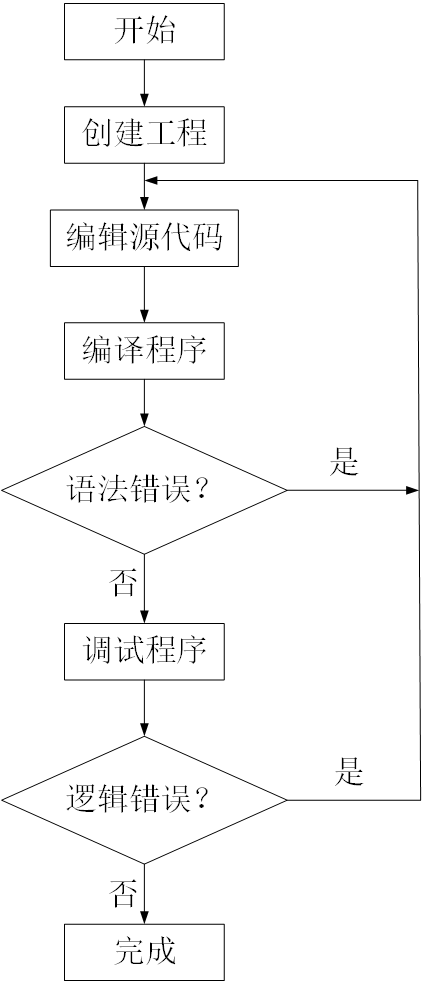
\includegraphics[width=0.45\textwidth]{debug_flowchart}
\end{figure}

\column{0.5\textwidth}
\begin{yellowblock}{说明}
\begin{enumerate}
  \item 建立工程、编写源代码
  \item 编译,编译器会指出具体的语法错误
  \item 改正语法错误
  \item {\color{red}调试程序,找出逻辑错误(监视窗口观察对象内容的变化)}
\end{enumerate}
\end{yellowblock}

\end{columns}
\end{frame}
%---------------------------------------------------------------------------------------------
\begin{frame}[fragile]{1.3 编译与调试程序}

\begin{columns}[t]
\column{0.8\textwidth}
\begin{blueblock}{\texttt{Visual Studio}\footnote{下载地址 https://visualstudio.microsoft.com/vs/community/}几个常用快捷键}

\begin{tabular}{ll}
  % after \\: \hline or \cline{col1-col2} \cline{col3-col4} ...
  \alert{\texttt{F5}} & 执行程序 \\
  \alert{\texttt{F7}} & 编译源文件 \\
  \alert{\texttt{F9}} & 添加断点 \\
  \alert{\texttt{F10}} & 单步执行一行代码 \\
  \alert{\texttt{F11}} & 进入函数体\\
\end{tabular}
\end{blueblock}
\pause
~\\
\begin{yellowblock}{建议}
	\begin{itemize}
		\item 遵循“编辑--编译--调试”的原则
		\item 养成调试程序的好习惯
	\end{itemize}
\end{yellowblock}

\end{columns}
\end{frame}


%%%%%%%%%%%%%%%%%%%%%%%%%%%%%%%%%%%%%%%%%%%%%%%%%%%%%%%%%%%%%%%%%%%%%%%%%%%%%%%%%%%%%%%%%%%%%%
\section{const修饰符}
%%%%%%%%%%%%%%%%%%%%%%%%%%%%%%%%%%%%%%%%%%%%%%%%%%%%%%%%%%%%%%%%%%%%%%%%%%%%%%%%%%%%%%%%%%%%%%

%---------------------------------------------------------------------------------------------
\begin{frame}[fragile]{2.4 常量修饰符和类型推导\normalsize{~---~const修饰符}}
对于存储圆周率$\pi$、自然对数e等常量的对象,我们不希望其内容发生变化。C++提供了关键字\alert{const}对对象的类型加以限制。

\begin{columns}[t]
\column{0.55\textwidth}
\begin{blueblock}{例如}
    \begin{lstlisting}
//圆周率用pi表示,即有时给常量取个名字更方便
const double pi = 3.14159;
int i = 100;
//利用对象 i 的值初始化 ci
const int ci = i;
    \end{lstlisting}
\end{blueblock}


\begin{greenblock}<3->{问题}
判断如下代码是否正确?
    \begin{lstlisting}
const int numStudent = 30;
numStudent = 50;
const double pi;
    \end{lstlisting}
\end{greenblock}

\column{0.4\textwidth}
\begin{yellowblock}<2->{说明}
\begin{itemize}
    \item const修饰的对象不能改变其内容,即不能对其进行写操作
    \item const对象创建时必须初始化
\end{itemize}
\end{yellowblock}
~\\
\begin{greenblock}<4->{答案}
\begin{itemize}
  \item 第二行代码错误:不能对 numStudent 进行写值操作
  \item 第三行代码错误:const 对象必须初始化
\end{itemize}
\end{greenblock}

\end{columns}
\end{frame}

\begin{frame}[fragile]
	\frametitle{4.2 指针\small{—\texttt{const}和指针}}
	% \framesubtitle{——\texttt{const}和指针}
	\begin{block}{\texttt{const}和指针}
		\begin{itemize}
			\item 可以用\texttt{const}修饰符,使其不能修改所指向对象的值,即\alert{指向const对象}的指针。
			      例如:\\
			      \begin{lstlisting}[basicstyle=\small\ttfamily]
const int ci = 10, cj = 1;
const int *ptrc = &ci; //ptrc 指向常量ci
        \end{lstlisting}
		\end{itemize}
	\end{block}
	\begin{exampleblock}{练习:}
		\ttfamily 下面语句有错误吗?若有,则错在哪里?
		\begin{columns}
			\begin{column}{0.4\linewidth}
				\begin{lstlisting}[basicstyle=\small\ttfamily]
    const int a = 30;
    const int *c = &a;
    *c = 100;

    \end{lstlisting}
			\end{column}
			\hfill
			\begin{column}{0.55\linewidth}
				\onslide<2->{答案:语句\texttt{*c = 100;}错误, 不能修改所指向对象的值}
			\end{column}
		\end{columns}
	\end{exampleblock}
\end{frame}

\begin{frame}[fragile]
	\frametitle{4.2 指针\small{—\texttt{const}和指针}}
	% \framesubtitle{——\texttt{const}和指针}
	\begin{block}{\texttt{const}指针}
		不允许改变指向的指针,语法格式:
		\begin{lstlisting}[basicstyle=\small\ttfamily]
int j = 0, i = 0;
int *const cptr = &i; //定义时初始化,cptr 只能指向对象i
cptr = &j;               //错误:不能改变cptr 的指向
*cptr = 10;              //正确:可以通过*cptr 修改其指向的对象i 的值
        \end{lstlisting}
	\end{block}
\end{frame}

\begin{frame}[fragile]
	\frametitle{4.2 指针\small{—\texttt{const}和指针}}
	% \framesubtitle{——\texttt{const}和指针}
	\ttfamily
	\begin{block}{指向\texttt{const}对象的\texttt{const}指针}
		\begin{lstlisting}[basicstyle=\small\ttfamily]
const int *const cptrc = &ci;//cptrc 是一个指向常量ci 的常量指针
    \end{lstlisting}
		\ttfamily 第一个~const~修饰符表明~cptrc~为一个指向~const~对象的指针,第二个~const~修饰符表明~cptrc~不能改变指向
	\end{block}
\end{frame}

%%%%%%%%%%%%%%%%%%%%%%%%%%%%%%%%%%%%%%%%%%%%%%%%%%%%%%%%%%%%%%%%%%%%%%%%%%%%%%%%%%%%%%%%%%%%%%
\section{auto类型推导}
%%%%%%%%%%%%%%%%%%%%%%%%%%%%%%%%%%%%%%%%%%%%%%%%%%%%%%%%%%%%%%%%%%%%%%%%%%%%%%%%%%%%%%%%%%%%%%
%---------------------------------------------------------------------------------------------
\begin{frame}[fragile]{2.4 常量修饰符和类型推导\normalsize{~---~类型推导}}
\begin{columns}[t]
\column{0.9\textwidth}
\begin{lstlisting}
int i = 0;
\end{lstlisting}对于上面这条代码,能否根据操作数0的类型(\texttt{int})自动推断出i的类型?
\pause
~\\
    \begin{greenblock}{答}
利用 \alert{auto},编译器可以根据初始值的类型自动推导出所需数据类型
    \begin{lstlisting}
auto pi=3.14159, rad=1.0;   // pi 和 rad 都为 double 类型
auto area=pi*rad*rad;       // area 为 double 类型
auto i=0, pi=3.14159;       // 错误:i 和 pi 的类型不一致
    \end{lstlisting}
    \end{greenblock}
\pause
    \begin{redblock}{注意}
\begin{itemize}
    \item 当用\texttt{auto}定义多个对象时,其显示类型必须一致,否则会报错
    \item \texttt{auto}不能肆意使用,否则会造成代码的可读性和可维护性下降,使用时需要权衡利弊
\end{itemize}
    \end{redblock}
\end{columns}
\end{frame}

%%%%%%%%%%%%%%%%%%%%%%%%%%%%%%%%%%%%%%%%%%%%%%%%%%%%%%%%%%%%%%%%%%%%%%%%%%%%%%%%%%%%%%%%%%%%%%
\section{引用}
%%%%%%%%%%%%%%%%%%%%%%%%%%%%%%%%%%%%%%%%%%%%%%%%%%%%%%%%%%%%%%%%%%%%%%%%%%%%%%%%%%%%%%%%%%%%%%

\begin{frame}[fragile]
	{4.1 引用}
	\begin{abstractblock}{引用}
		\begin{itemize}
			\item 为已创建的对象取一个\alert{别名}
			\item 只将别名绑定到所引用的对象,对象的内容不会复制给引用
			\item 函数间共享局部对象的重要途径,对于提高程序的效率有重要作用
		\end{itemize}
	\end{abstractblock}
\pause
	\begin{block}{语法}
		\begin{lstlisting}[basicstyle=\small\ttfamily]
int counter = 0;
int &refCnt = counter;  //refCnt引用counter对象的内容
int &refCnt2;             //错误:定义引用时必须和一个对象绑定
        \end{lstlisting}
		\begin{lstlisting}[basicstyle=\small\ttfamily]
refCnt = 2;       //修改了counter所在的内存空间的内容
int i = refCnt;//通过引用读取counter对象的内容,并初始化对象i
        \end{lstlisting}
	\end{block}
\end{frame}

\begin{frame}[fragile]
	{4.1 引用}
	\noindent 定义引用时,除了需要初始化外,还需要注意以下几点:
	\begin{block}{1. 定义多个引用时,每个引用必须用~\texttt{\&}~标明:}
		\begin{lstlisting}[basicstyle=\small\ttfamily]
int i = 0;
int &r1 = i, j = 0, &r2 = r1; //r1 和 r2 都是 i 的引用,而 j 是 int 类型
            \end{lstlisting}
	\end{block}
	\begin{block}{2. 只能引用同类型的对象:}
		\begin{lstlisting}[basicstyle=\small\ttfamily]
double d = 0;
int &r3 = d; //错误:r3 只能引用 int 类型对象
            \end{lstlisting}
	\end{block}
	\begin{block}{3. 引用的对象必须是非\texttt{const}左值:}
		\begin{lstlisting}[basicstyle=\small\ttfamily]
int i = 0; const int ci = 0;
int &r4 = 100, &r5 = i+1, &r6 = ci; //错误:只能引用非 const 左值
            \end{lstlisting}
	\end{block}
\end{frame}

\begin{frame}[fragile]
    {5.3 参数传递\small{~---~引用传递}}
\begin{block}{引用传递}
形参是实参的引用
\begin{itemize}
  \item 引用类型;
  \item 通过形参改变实参的值。
\end{itemize}
\end{block}
\begin{blueblock}<2->{引用传递的例子}\vspace{-1.5mm}\begin{lstlisting}
void Swap(int &x, int &y) {//x和y分别是实参i和j的别名
    int z(x);
    x = y;
    y = z;
} //交换x和y所绑定的对象的值
int main() {
    int i(4), j(5);
    Swap(i, j);
    cout << "i=" << i << ",j=" << j << endl;//输出i=4,j=5
    return 0;
}
\end{lstlisting}\vspace{-1.5mm}
\end{blueblock}

\end{frame}

\end{document}
